\documentclass[a4paper,14pt]{extarticle}

\usepackage[left=30mm, right=10mm, top=20mm, bottom=20mm]{geometry}

\usepackage[T2A]{fontenc}
\usepackage[utf8]{inputenc}
\usepackage[russian]{babel}
\usepackage{tempora}
\usepackage{type1cm}
\usepackage{indentfirst}

\usepackage{minted}
\usepackage{xcolor}

\usepackage{siunitx}
\usepackage{booktabs}
\usepackage{multirow}


\usepackage{csquotes}
\usepackage[
    parentracker=true,
    backend=biber,
    style=gost-numeric,
    sorting=nty
]{biblatex}

\usepackage[nodisplayskipstretch]{setspace}
\usepackage[none]{hyphenat}
\usepackage{fancyhdr}
\usepackage{titlesec}
\usepackage{tocloft}

\usepackage{amssymb}
\usepackage{amsmath}
\usepackage{tikz}
\usepackage{pgfplots}
\usepackage{graphicx}
\usepackage{caption}
\usepackage{subcaption}
\usepackage[hidelinks]{hyperref}
\usepackage[russian]{cleveref}
\usepackage{bookmark}

\pgfplotsset{compat=1.18}

\onehalfspacing
\sloppy

\pagestyle{fancy}
\fancyhf{}
\fancyfoot[R]{\thepage}
\renewcommand{\headrulewidth}{0pt}

\definecolor{codebg}{rgb}{0.12,0.12,0.14}
\definecolor{codeframe}{rgb}{0.40,0.40,0.45}
\definecolor{keywordcolor}{rgb}{0.45,0.65,1.0}
\definecolor{stringcolor}{rgb}{1.0,0.55,0.45}
\definecolor{commentcolor}{rgb}{0.55,0.75,0.60}
\definecolor{textcolor}{rgb}{0.90,0.90,0.90}

\renewcommand{\theFancyVerbLine}{
	\sffamily\small\color{black}\arabic{FancyVerbLine}
}

\setminted{
    bgcolor=codebg,
	fillcolor=codebg,
	framesep=1em,
	frame=single,
    rulecolor=\color{codeframe},
    fontsize=\normalsize,
    baselinestretch=1.1,
    linenos,
    numbersep=6pt,
    tabsize=4,
    breaklines,
    breakbytoken,
	breaksymbolleft={},
    autogobble,
    showspaces=false,
    showtabs=false,
}

\usemintedstyle{lightbulb}
\setmintedinline{
    bgcolor=codebg
}

\makeatletter
\setlength{\@fptop}{0pt}
\setlength{\@fpsep}{8pt}
\setlength{\@fpbot}{0pt plus 1fil}
\makeatother

\newcommand{\circledequals}{\mathbin{\tikz \node[draw,circle,inner sep=1pt] {$=$};}}

\DeclareMathOperator{\sgn}{sgn}

\begin{document}
    \begin{titlepage}
		\centering
		
		
\includegraphics{images/FEFU-logo.jpg}\\
		МИНИСТЕРСТВО ОБРАЗОВАНИЯ И НАУКИ РОССИЙСКОЙ ФЕДЕРАЦИИ\\
		Федеральное государственное автономное образовательное учреждение высшего образования\\
		\textbf{«Дальневосточный федеральный университет»}

		\rule{\linewidth}{0.8mm}\\[0.3cm]
		
		\textbf{ИНСТИТУТ МАТЕМАТИКИ И КОМПЬЮТЕРНЫХ ТЕХНОЛОГИЙ}\\
		\textbf{Кафедра математического и компьютерного моделирования}\\
		\vspace*{0.9cm}
		
		Кулахсзян Сергей Грайрович\\
        \vspace*{0.3cm}

		ЛАБОРАТОРНАЯ РАБОТА № 1 \\
        ЗАДАЧА № 8 \\
		\vspace*{0.5cm}

		\textbf{Задачи на площадь криволинейной трапеции}\\
		\vspace*{0.5cm}

		Направление подготовки 02.03.01сцт Сквозные цифровые технологии,\\ 
        бакалавриатская программа «Математика и компьютерные науки»\\ 
        Очной формы обучения\\
		\vspace{1.5cm}

		
		\vfill
		\centering
		г. Владивосток\\
		2026
	\end{titlepage}

    \tableofcontents
    \thispagestyle{empty}

	\newpage
    \pagenumbering{arabic}
    \setcounter{page}{3}
    \section{Постановка задачи}

    Даны кривые со следующим свойством: если через любую точку данной кривой провести прямые, параллельные осям координат, до пересечения с этими осями, то площадь полученного прямоугольника делится кривой в отношении 1:3. В таком случае кривая находится внутри прямоугольника, у которой одна из вершин в начале координат, а противоположная -- в точке $(x_0; y_0)$, где $x_0 \neq 0, y_0 \neq 0$.

    В таком случае площадь прямоугольника равна $|x_0 y_0|$, площадь трапеции -- $\displaystyle \sgn(x_0) \int_{0}^{x_0} |y(x)| dx$. При этом площадь трапеции должна составлять $\displaystyle \frac{1}{4}$ или $\displaystyle \frac{3}{4}$ от площади прямоугольника.

    В таком случае площадь трапеции к площади прямоугольника соотносится следующим образом:
    \begin{equation} \label{integral_equation}
        \left[
            \begin{array}{l}
                 \displaystyle 4 \sgn(x y) \int_{0}^{x} y(t) dt = \sgn(x y) xy \\
                 \displaystyle 4 \sgn(x y) \int_{0}^{x} y(t) dt = 3 \sgn(x y) xy 
            \end{array}
        \right. \Longleftrightarrow 
        \left[
            \begin{array}{l}
                 \displaystyle 4 \int_{0}^{x} y(t) dt = xy \\
                 \displaystyle 4 \int_{0}^{x} y(t) dt = 3 xy 
            \end{array}
        \right..
    \end{equation}

    Дифференцируя уравнения (\ref{integral_equation}) получаем следующую математическую модель:
    \begin{equation} \label{model}
        \begin{cases}
            \left[
                \begin{array}{l}
                     \displaystyle 3y = xy' \\
                     \displaystyle y = 3xy'
                \end{array}
            \right. \\
            y(1) = -1
        \end{cases}.
    \end{equation}

    \newpage
    \section{Решение}
    \subsection{Аналитическое решение}
    
    Уравненение (\ref{model}) имеет следующее решение:
    \[
        \begin{aligned}
            3y = xy' &\quad\quad& y = 3xy'  \\
            \displaystyle \frac{dy}{y} = \frac{3 dx}{x} &\quad\quad& \displaystyle \frac{dy}{y} = \frac{dx}{3x} \\
            \ln y = 3 \ln x + \ln c &\quad\quad& \ln y = \displaystyle \frac{1}{3} \ln x + \ln c \\
            y = cx^3 &\quad\quad& y = c\sqrt[3]{x}
        \end{aligned}
    \]
    \begin{equation}\label{analytical_solution}
        \left[
            \begin{array}{l}
                y = -x^3 \\ 
                y = -\sqrt[3]{x}
            \end{array}
        \right..
    \end{equation}

    \subsection{Численное решение}

    Для численного решения уравнений был применён метод Рунге-Кутта 4-го порядка, который имеет погрешность $O(h^4)$: \\
    $\displaystyle
    y_{i + 1} = y_i + \frac{h}{6} (k_1 + 2k_2 + 2k_3 + k_4), \\
    k_1 = f(x_i, y_i), \\
    k_2 = f \left( x_i + \frac{h}{2}, y_i + \frac{h}{2} k_1 \right), \\
    k_3 = f \left( x_i + \frac{h}{2}, y_i + \frac{h}{2} k_2 \right), \\
    k_4 = f(x_i + h, y_i + h k_3).
    $

    Вычисление было произведено на отрезке $[1; 10]$ при значениях $N = 10; 100; 1000$.

    \newpage
    \section{Результаты}

    В ходе выполнения были получены следующие результаты представленные на графиках:

    \begin{figure}[htbp]
        \centering
        \begin{subfigure}[b]{\textwidth}
            \centering
            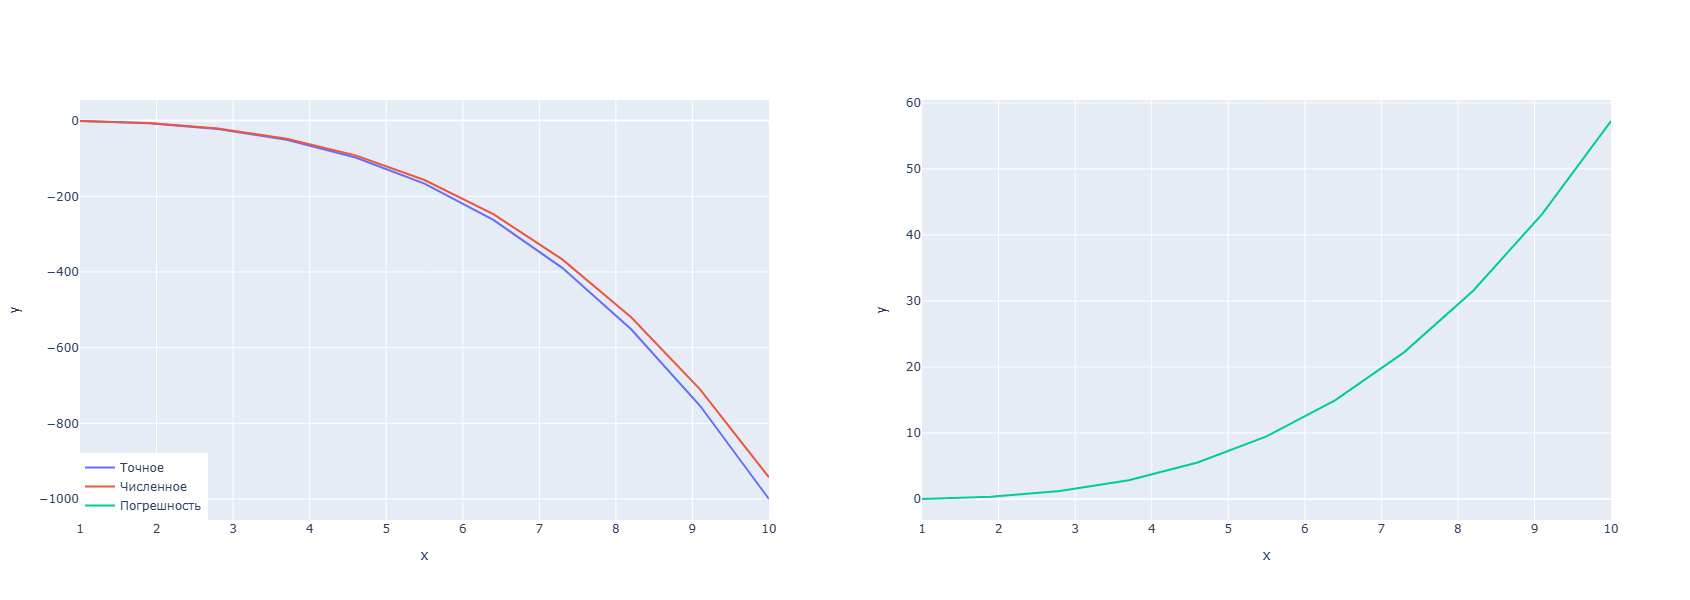
\includegraphics[width=\textwidth]{images/1_10.png}
            \caption{$3y = xy'$}
        \end{subfigure}
        \hfill
        \begin{subfigure}[b]{\textwidth}
            \centering
            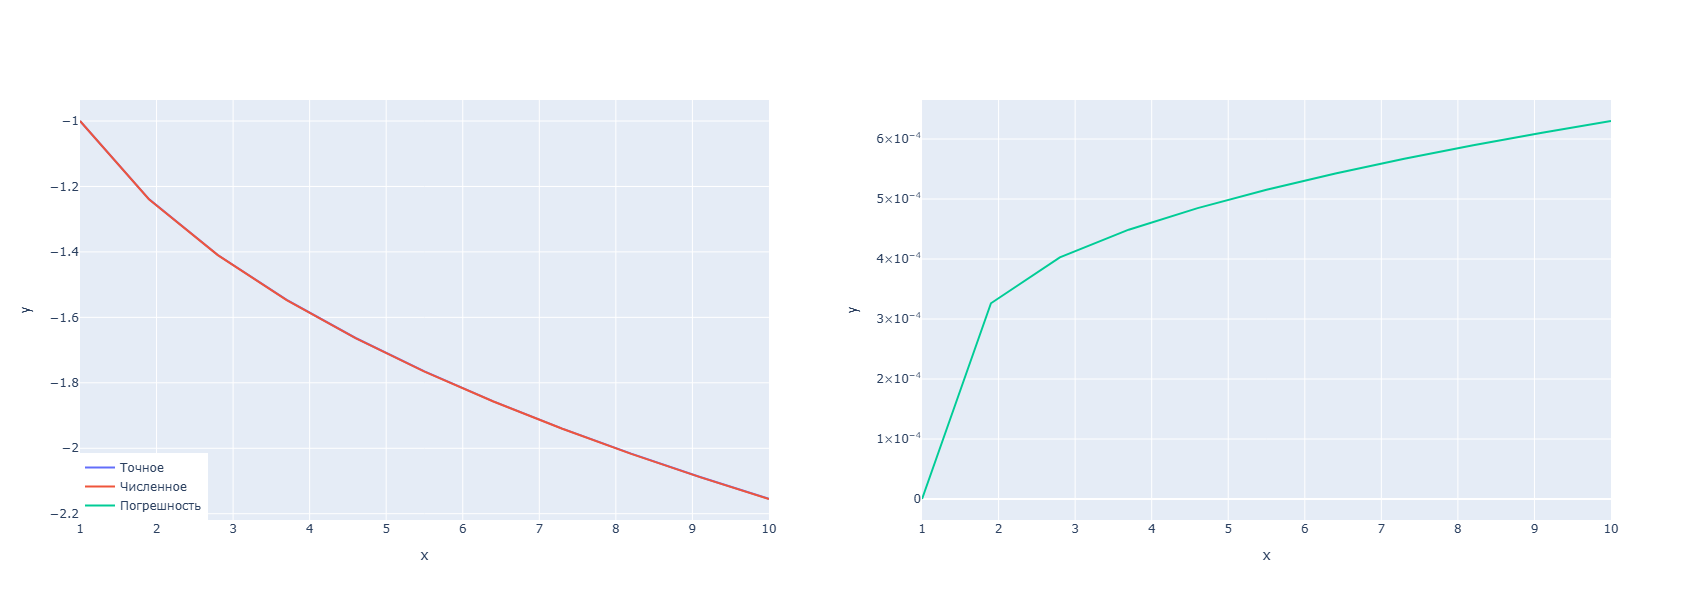
\includegraphics[width=\textwidth]{images/2_10.png}
            \caption{$y = 3xy'$}
        \end{subfigure}
        
        \caption{Тестирование решения при $N = 10$}
        \label{n_10}
    \end{figure}

    \begin{figure}[htbp]
        \centering
        \begin{subfigure}[b]{\textwidth}
            \centering
            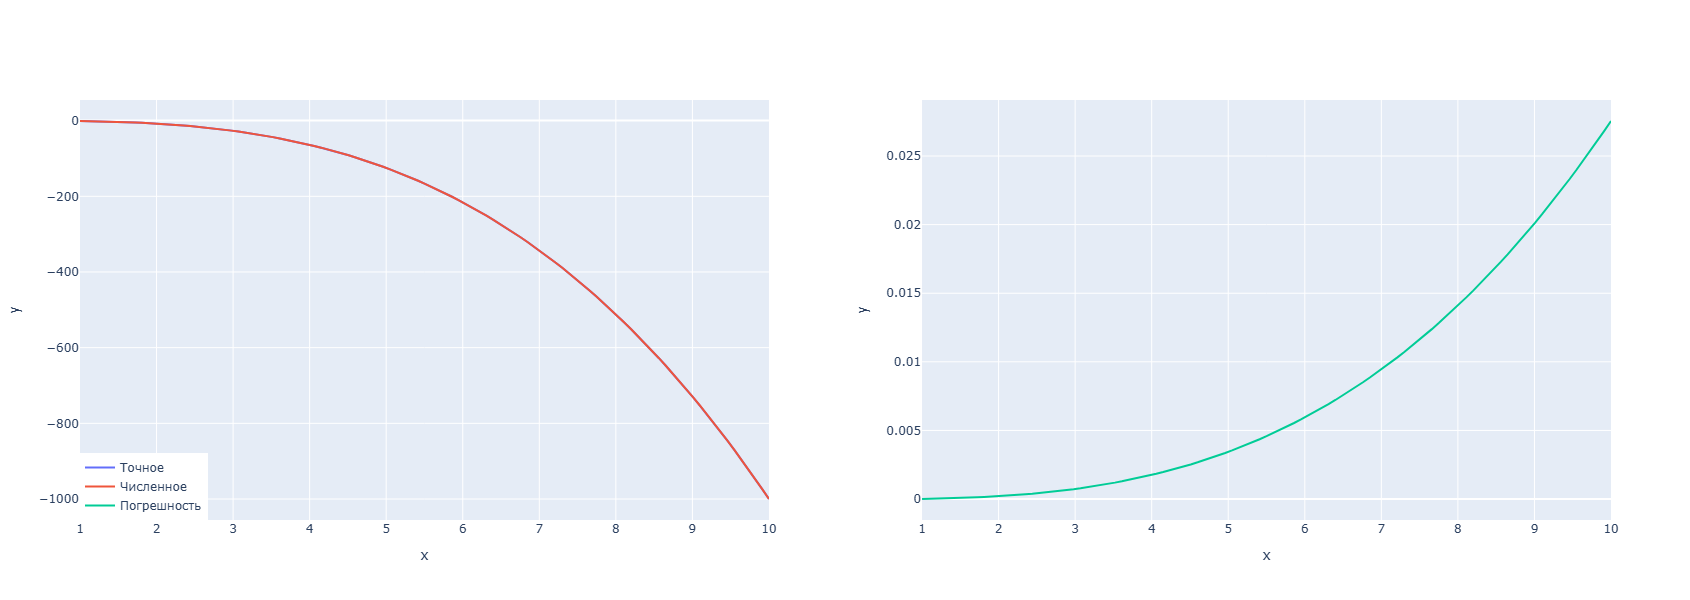
\includegraphics[width=\textwidth]{images/1_100.png}
            \caption{$3y = xy'$}
        \end{subfigure}
        \hfill
        \begin{subfigure}[b]{\textwidth}
            \centering
            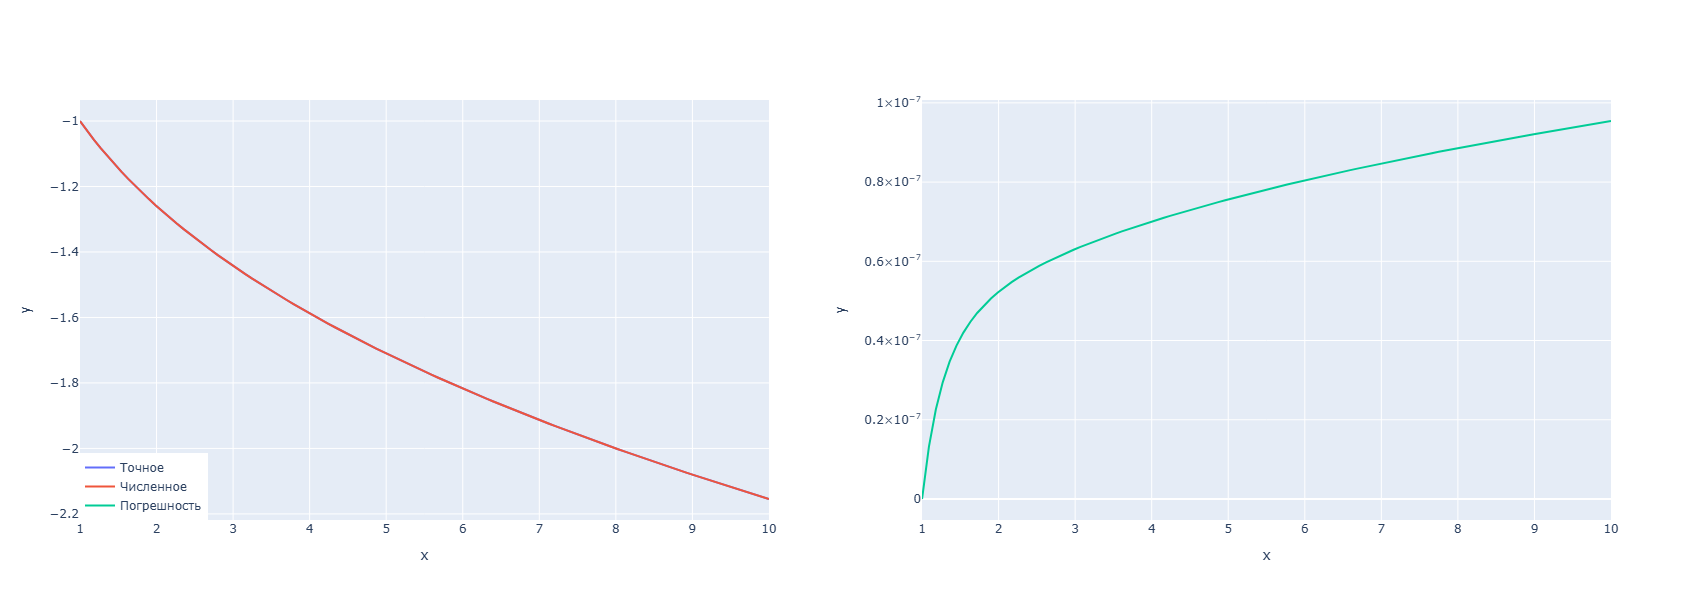
\includegraphics[width=\textwidth]{images/2_100.png}
            \caption{$y = 3xy'$}
        \end{subfigure}
        
        \caption{Тестирование решения при $N = 100$}
        \label{n_100}
    \end{figure}

    \begin{figure}[htbp]
        \centering
        \begin{subfigure}[b]{\textwidth}
            \centering
            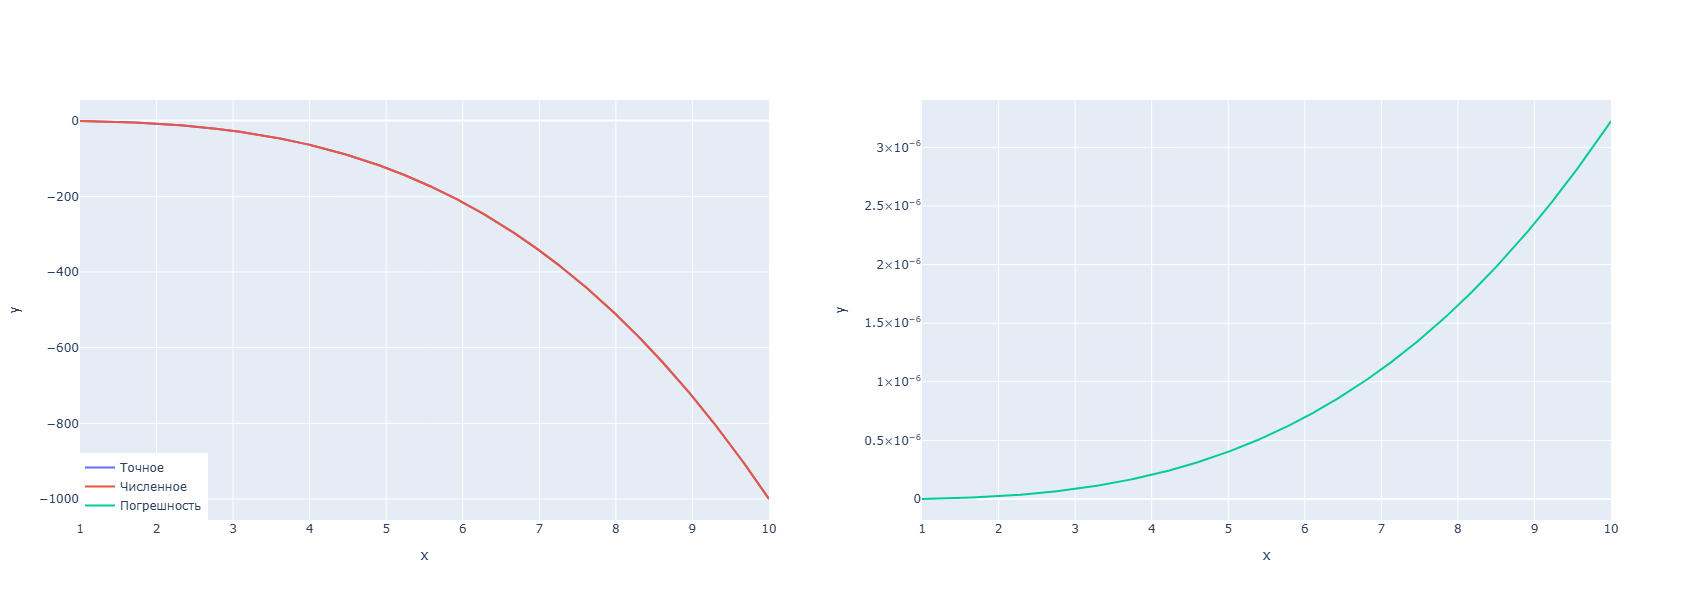
\includegraphics[width=\textwidth]{images/1_1000.png}
            \caption{$3y = xy'$}
        \end{subfigure}
        \hfill
        \begin{subfigure}[b]{\textwidth}
            \centering
            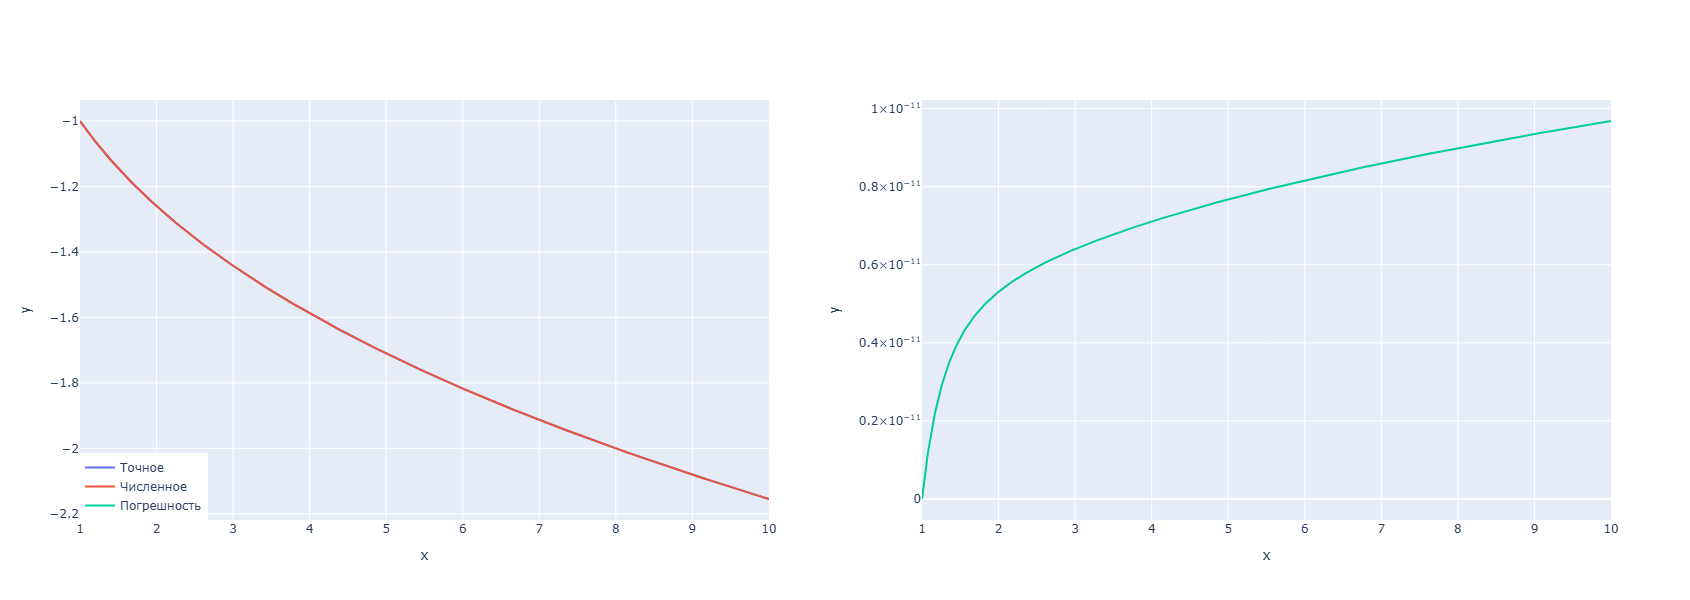
\includegraphics[width=\textwidth]{images/2_1000.png}
            \caption{$y = 3xy'$}
        \end{subfigure}
        
        \caption{Тестирование решения при $N = 1000$}
        \label{n_1000}
    \end{figure}

    \newpage
    \section{Заключение}

    В ходе лабораторной работы была рассмотрена и решена задача о расчёте площади криволинейной трапеции. Сравнение численных и аналитических решений, приведённое на графиках (\cref{n_10}, \cref{n_100}, \cref{n_1000}), показало, что при увеличении числа узлов сетки численное решение всё точнее приближается к аналитическому.
\end{document}